\documentclass{standalone}
\usepackage{tikz}
\usetikzlibrary {angles,quotes}
\begin{document}
    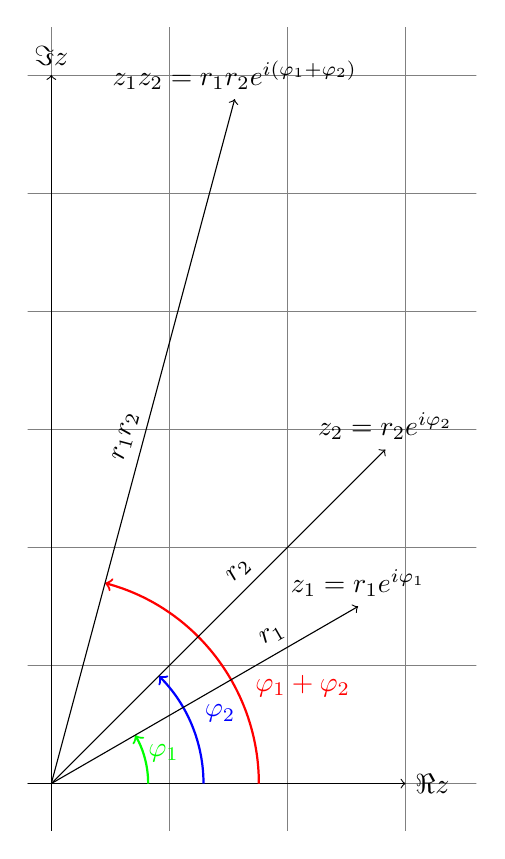
\begin{tikzpicture}[scale=3]
        % selecting the first quadrant
        \clip (-0.1,-0.2) rectangle (1.8,3.2);
        % setting up the Cartesian Grid. Note "help lines" = "gray, very thin"
        \draw[step=.5cm,help lines] (-1.6,-1.6) grid (2.5,3.5);
        % setting up the real and imaginary axis. 
        \draw[->] (-1.5,0) -- (1.5,0) coordinate (x axis) node[right] {$\Re z$};
        \draw[->] (0,-1.5) -- (0,3) coordinate (y axis) node[above] {$\Im z$};

        \coordinate (origin) at (0,0);
        \coordinate (A) at (2,0);
        \coordinate (B) at (75:2);

        \draw pic [draw=red,->,thick,angle eccentricity=1.2,angle radius=75,"{$\varphi_1+\varphi_2$}"{shift={+(-45:27.5pt)}, red}] {angle = A--origin--B};

        \coordinate (C) at (1.5,0);
        \coordinate (D) at (45:1.5);

        \draw pic [draw=blue,->,thick, angle eccentricity=1.2,angle radius=55, "$\varphi_2$"{blue}] {angle = C--origin--D};

        \coordinate (E) at (1,0);
        \coordinate (F) at (30:1cm);
      
        \draw pic [draw=green,->,thick, angle eccentricity=1.2,angle radius=35, "$\varphi_1$"{green}] {angle = E--origin--F};

        % z_1
        \draw[->] (0,0) -- (30:1.5) node[near end, above, sloped] {$r_1$} node[at end, above] {$z_1=r_1e^{i\varphi_1}$} coordinate (z1);

        % z_2
        \draw[->] (0,0) -- (45:2) node[pos=0.6, above, sloped] {$r_2$} node[at end, above] {$z_2=r_2e^{i\varphi_2}$} coordinate (z2);

        % z_1*z_2
        \draw[->] (0,0) -- ({30+45:1.5*2}) node[midway, above, sloped] {$r_1 r_2$} node[at end, above] {$z_1 z_2=r_1 r_2 e^{i(\varphi_1 + \varphi_2)}$};

    \end{tikzpicture}
\end{document}
